% \documentclass{article}


\documentclass[twoside]{article}

\usepackage[math]{kurier}
\usepackage[sc]{mathpazo}
\renewcommand{\sfdefault}{kurier}
\usepackage[utf8]{inputenc}
\usepackage{graphicx}
\usepackage{caption}
\usepackage{hyperref}
\usepackage{subcaption}
\usepackage{wrapfig}
\usepackage{amsmath}
\usepackage{enumitem}
\usepackage{float}
\usepackage{framed} % or, "mdframed"
\usepackage[framed]{ntheorem}
\newframedtheorem{frm-def}{Definition}
\usepackage{graphics}
\setlength{\oddsidemargin}{0.25 in}
\setlength{\evensidemargin}{-0.25 in}
\setlength{\topmargin}{-0.6 in}
\setlength{\textwidth}{6.5 in}
\setlength{\textheight}{8.5 in}
\setlength{\headsep}{0.75 in}
\setlength{\parindent}{0 in}
\setlength{\parskip}{0.1 in}


\newcounter{lecnum}
\renewcommand{\thepage}{\thelecnum-\arabic{page}}
\renewcommand{\thesection}{\thelecnum.\arabic{section}}
\renewcommand{\theequation}{\thelecnum.\arabic{equation}}
\renewcommand{\thefigure}{\thelecnum.\arabic{figure}}
\renewcommand{\thetable}{\thelecnum.\arabic{table}}


\newcommand{\lecture}[3]{
   \pagestyle{myheadings}
   \thispagestyle{plain}
   \newpage
   \setcounter{lecnum}{#1}
   \setcounter{page}{1}
   \noindent
   \begin{center}
   \framebox{
      \vbox{\vspace{2mm}
    \hbox to 6.28in { {\bf \sffamily AA 274: Principles of Robotic Autonomy
                        \hfill Winter 2019} }
       \vspace{4mm}
       \hbox to 6.28in { {\sffamily{\Large \hfill Lecture #1: #2  \hfill}} }
       \vspace{2mm}
       %\hbox to 6.28in { {\it \hfill Scribes: #4} }
      \vspace{2mm}}
   }
   \end{center}
   \markboth{Lecture #1: #2}{Lecture #1: #2}

   \vspace*{4mm}
}


\begin{document}

\lecture{1}{Mobile Robot Kinematics}{}{}

The following notes summarize the first lecture of AA 274: Principles of Robotic Autonomy. This lecture covers two introductory materials (Mobile Robot Kinematics and Motion Control), is organized into meaningful sections, and is annotated with formal definitions, graphics and literature references.

\section*{Course Introduction}

This goal of this course is to learn the theoretical, algorithmic and implementation aspects of the
main techniques for robot autonomy. The four following pillars of the ``autonomy stack" will be covered:

\begin{enumerate}
    \item motion control (2 lectures);
    \item perception, from classic to deep learning approaches (6 lectures);
    \item localization and SLAM (4 lectures);
    \item planning, decision making and system architecting (4 lectures).
\end{enumerate}

In addition to covering the above theoretical topics on robot autonomy, the course will also emphasize  hands on practical experience - this will happen through the extensive use of the Robotic Operating System (ROS) in both assignments and the final project. For more details on ROS, see lecture 2.

\section*{Lecture 1 Introduction}

Lecture 1 will describe kinematic constraints on mobile robots, and different robot wheel configurations. We will merge these concepts to describe a few wheeled robot kinematic models. Outlined below
\begin{enumerate}
    \item Kinematic Constraints
    \begin{enumerate}
        \item Holonomic Constraints
        \item Nonholonomic Constraints
    \end{enumerate}
    \item Wheel Configurations
    \begin{enumerate}
        \item Standard Wheels
        \item Castor Wheels
        \item Omni-directional Wheels
    \end{enumerate}
    \item Mobile Robot Models
    \begin{enumerate}
        \item Unicycle (a.k.a. "differential drive")
        \item Tricycle (simple car)
    \end{enumerate}
\end{enumerate}

In this class, an emphasis will be placed on mobile robots and vehicles as opposed to stationary machines. With mobile robots, the focus is on motion and trajectories rather than configurations and interactions with the environment. As such, we need to consider the dynamics and kinematic constraints that govern the motion of each robot.

\section*{Kinematic Constraints}
\subsection*{Holonomic Constraints}

The motion state, or configuration, of a robot at any point in time is given by the configuration vector \cite{ssvo}:

$$
\xi = [\xi_1, \xi_2, \ ... \  \xi_n]^T
$$

For example, a differential drive robot would have $ \xi = [x, y, \theta]^T, $ denoting a 2D position and an orientation angle.

A time series of changing configurations $ \xi(t) $ is called a trajectory, and the set of differential equations $ \dot{\xi} = f(\xi,u) $ that govern the robot's motion is known as the robot's dynamic model. We will see later that general dynamic models are already known for most robots. They can, however, also be derived from any given robot's kinematic constraints.

Kinematic constraints take the form of mathematical statements involving $\xi$, that must hold at all times during robot operation. We introduce some formal notation and terminology at this point:

\begin{frm-def}[Holonomic Constraints]
A kinematic constraint is holonomic if it can be expressed as:
$$
h_i(\xi) = 0,\;\;\textup{for}\;\;i = 1,...,k < n
$$
Each holonomic constraint reduces the number of degrees of freedom of the robot's configuration by 1 (i.e. it reduces the space of accessible configurations of the vehicle to an \textit{n-k} dimensional subset.
\end{frm-def}

\begin{frm-def}[Kinematic Constraints]
A mobile robot system with $n$ degrees of freedom has kinematic constraints that can be described in a general way as follows:
$$
a_i (\xi, \dot{\xi})=0,\;\;\textup{for}\;\;i = 1,...,k < n
$$
A subcategory of kinematic constraints can be expressed in the Pfaffian form:
$$
a_i(\xi) \cdot \dot{\xi} = 0,\;\;\textup{for}\;\;i = 1,...,k < n
$$
\end{frm-def}

We can see that a holonomic constraint always also imposes a kinematic constraint:
$$
h_i(\xi) = 0 \Rightarrow \frac{d\,h_i(\xi)\, }{dt} = \frac{\partial\,h_i(\xi)}{\partial \xi} \dot{\xi} = 0,\;\;\textup{for}\;\;i = 1,...,k < n
$$
However, the converse is generally not true \cite{ssvo}.

\subsection*{Nonholonomic Constraints}

The general kinematic constraint in the form $ a_i (\xi, \dot{\xi}) $ can either be a holonomic or a nonholonomic constraint. It is holonomic if it can be integrated to the holonomic form of $ h_i(\xi) = 0 $. Otherwise, it is nonholonomic \cite{ssvo}.

In practice, both types of constraints affect the system differently: holonomic constraints reduce accessibility of the robot by limiting the robot configuration to a lower-dimensional subspace (each constraint removes one degree of freedom), whereas nonholonomic constraints do not limit accessibility at all; instead, they constrain the possible velocities at each configuration state. In particular, Pfaffian form constraints $ a_i(\xi) \cdot \dot{\xi} = 0 $ allow only velocities from the null space of $ a_i (\xi) $.

A kinematic system with any nonholonomic constraints is denoted as a nonholonomic mechanical system.

\subsubsection*{Example: Single No Slip Disk \cite{ssvo}}

\begin{figure}[H]
\centering
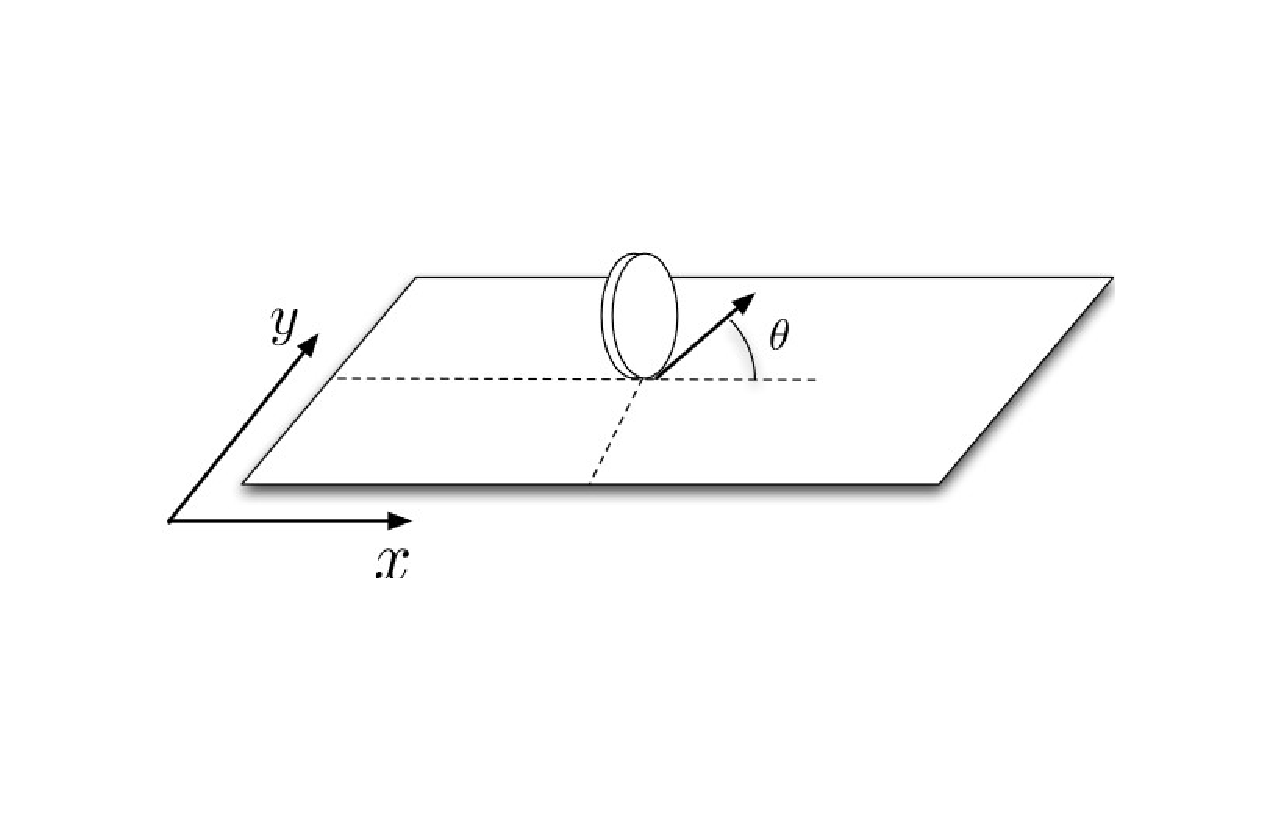
\includegraphics[width=0.35\textwidth]{Slip_Disk_Example}
\caption{Single No Slip Disk Diagram}
\end{figure}

We consider a disk rolling on its edge to demonstrate a nonholonomic system. Like a differential drive robot, the configuration vector of this system is $ \xi = [x, y, \theta]^T $. The kinematic constraint on this system is the no slip constraint, i.e. the disk cannot move laterally - only longitudinally along its orientation.

To formulate this constraint mathematically, we express the two orthogonal directions like this:

\[ d_{long} =
\begin{pmatrix} \cos \theta \\ \sin \theta \end{pmatrix}
\perp
d_{lat} =
\begin{pmatrix} \sin \theta \\ -\cos \theta \end{pmatrix}
\]

We can enforce the no slip condition with a dot product statement between the velocity vector and $ d_{lat} $ as follows:

$$
[\dot{x},  \dot{y}] \begin{pmatrix} \sin \theta \\ -\cos \theta \end{pmatrix} = 0 \iff
[\sin \theta, -\cos \theta, 0] \dot{\xi} = 0
$$

This is a nonholonomic constraint in Pfaffian form. In this system there is no loss of accessibility.

The example shows that wheeled vehicles are generally nonholonomic, meaning they can reach any configuration $[x,y,\theta]^T$ but will have constrained trajectories to get there. A common holonomic system, on the other hand, would be a robotic arm that cannot reach any possible configuration due to mechanical interactions. In this case, its joints may constrain it such that some configurations are unreachable.

\subsection*{Types of wheels}

There are four main wheel types in mobile robotics. Since they are different in the way they constrain the robot's motion, knowing them is important to finding out the kinematic constraints and dynamic model of the vehicle.

The \textbf{Standard Wheel} is the most ubiquitous of the wheel types. Its defining property is that the wheel is mounted on the robot's frame directly above the wheel's point of contact with the ground. They can either be of fixed orientation, or they can be fitted to be steerable\cite{sns}.

\begin{figure}[H]
\centering
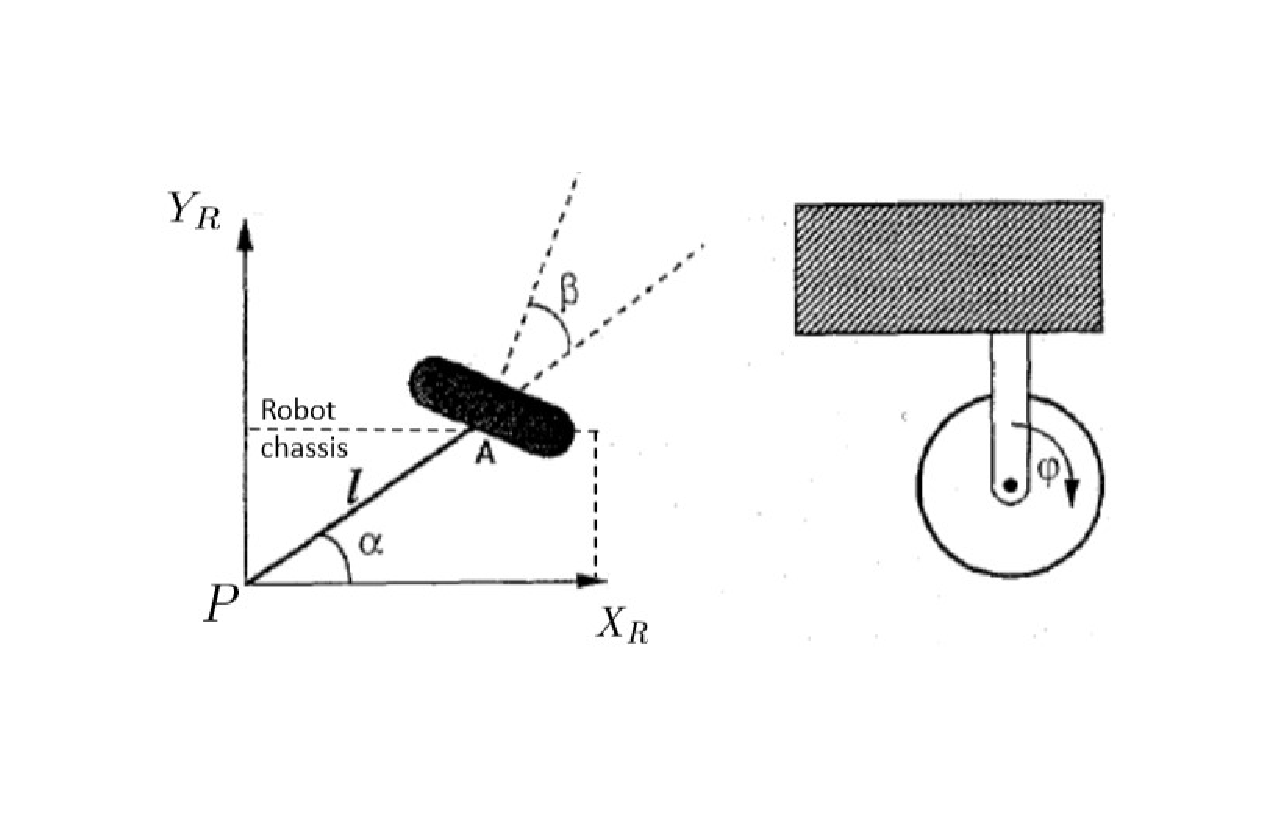
\includegraphics[width=0.6\textwidth]{Standard_Wheel}
\caption{Standard Wheel}
\end{figure}


The \textbf{Castor Wheel} differs from the fixed wheel in that it is mounted on the robot in an off-centered position and always fastened to a rotating axis. The wheel's orientation is then either actively steered or passively governed by the robot's motion. The main advantage of the Castor Wheel is that the off-centered axis of rotation essentially allows the wheel to circumvent the no-slip constraint. Of course, it still cannot achieve true omnidirectional motion because it can only exert force along its orientation\cite{sns}.

\begin{figure}[h]
\centering
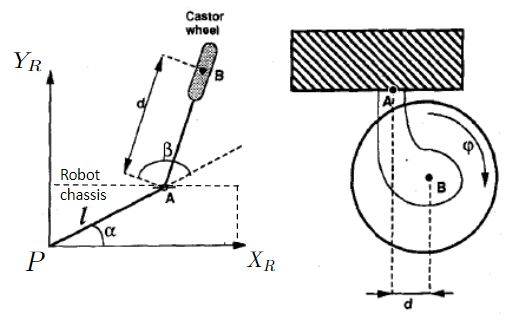
\includegraphics[width=0.4\textwidth]{cast}
\caption{Castor Wheel}
\end{figure}

The \textbf{Swedish Wheel} and the \textbf{Spherical wheel} are special wheel designs that both achieve omnidirectional motion in different ways. The Swedish Wheel is a big wheel with smaller rollers mounted on the rim allowing active movement in all directions\cite{sns}. The Spherical Wheel uses a different concept, where the "wheel" itself is actually ball-shaped. This wheel is suspended in a cage where it is in contact with a series of small motors that can turn the sphere to roll in any direction. They are quite rare however, so they will not play a large part in this class.

\begin{figure}[H]
\centering
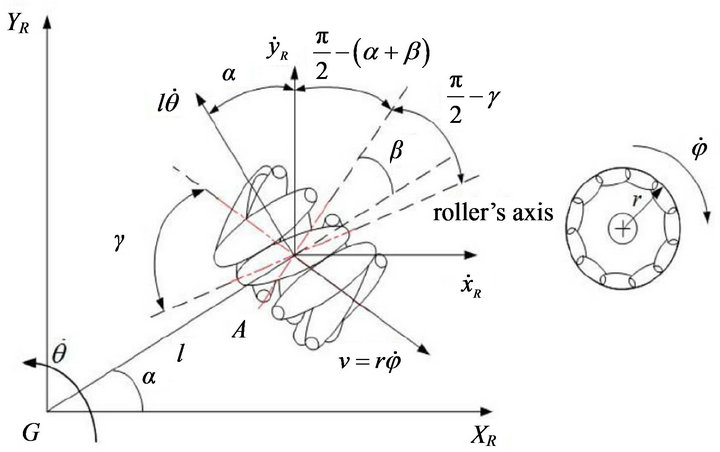
\includegraphics[width=0.5\textwidth]{swedish}
\caption{Omnidirectional Swedish Wheel \cite{swed}}
\end{figure}

\subsection*{Kinematic Models and Degree of Mobility}

By putting together all the constraints that arise from the no slip conditions, we can come up with a kinematic model of our robot. While we do not have to do this in this class, to derive the kinematic model for your given robot, you would compile the no slip constraints into a matrix, then look at the null space of that constraint matrix. This will tell you the set of possible velocities of your robot. The reason the null space of the constraint matrix forms the set of possible velocities is that the no slip conditions each impose a constraint in the Pfaffian form $$a_i(\xi) \cdot \dot{\xi} = 0.$$ Thus it is possible to reach a given velocity if and only if it is orthogonal to each row of the constraint matrix, or equivalently if it lies in the null space of the constraint matrix.

More specifically, a nonholonomic constraint matrix $C_1(\beta_s)$ is derived by stacking all the no slip conditions for the fixed wheels and steerable wheels:
$$C_1(\beta_s)= \begin{bmatrix}
           C_{1f} \\
           C_{1s}(\beta_s) \\
         \end{bmatrix}$$
where $C_{1f}$ is the matrix of no slip conditions for the fixed wheels and $C_{1s}(\beta_s)$ is the matrix of no slip conditions for the steerable wheels, which are steerable by the wheel angle $\beta_s$. The dimension of the null space of $C_1(\beta_s)$ determines the number of degrees of freedom the robot can move in by manipulating the wheel velocities, also known as the robot's degree of mobility $\delta_m$. The possible range of mobility values for any robot is $0 \leq \delta_m \leq 3.$ The degree of mobility is $\delta_m=3$ only if there are no independent kinematic constraints, i.e. if there are neither fixed nor steerable wheels attached to the robot. A degree of mobility of $\delta_m=0$ is only possible if there are three independent kinematic constraints (e.g. if the robot has three fixed wheels at different angles). In this case, the robot can not move in any direction.

By finding the null space of the nonholonomic constraint matrix you can express the set of possible velocities in a parameterized form. This is what is known as a kinematic model. We will use some simple kinematic models in this class to describe the motion of our mobile robot:

\subsubsection*{"Unicycle" (a.k.a. "differential drive") Model:}

This configuration type utilizes two rear standard wheels and an optional passive wheel in the front of the vehicle. In order to achieve rotation, the unicycle model makes use of differential drive by controlling the rate/direction of rotation for each wheel independently\cite{sns}.

\begin{figure}[H]
\centering
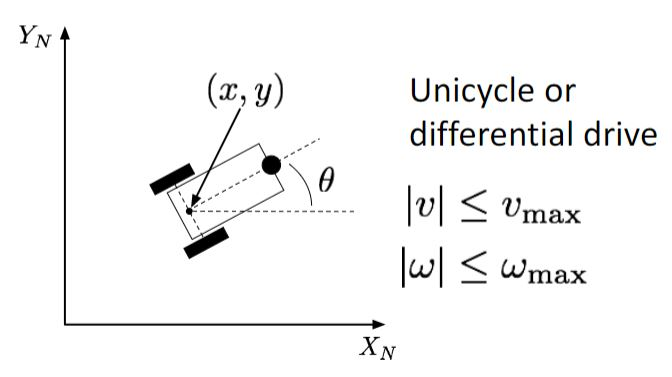
\includegraphics[width=0.35\textwidth]{unicycle}
\caption{Unicycle Model}
\end{figure}

The kinematic model of unicycle robots is as follows:

\[ \begin{pmatrix}
\dot{x} \\ \dot{y} \\ \dot{\theta}
\end{pmatrix} =
\begin{pmatrix} \cos \theta \\ \sin \theta \\ 0 \end{pmatrix} v + \begin{pmatrix} 0 \\ 0 \\ 1 \end{pmatrix} w
\]
This kinematic model is governed by the no lateral slip and pure rolling constraints of the fixed unicycle wheel. The differential-drive robot, although mechanically different, yields the same kinematic model. This is because the collection of constraints on a differential-drive robot can be combined to form one independent constraint. First, the passive wheel is free to move in any direction and can be ignored. Second, the two fixed drive wheels are parallel, therefore, the constraints do not allow the robot to move orthogonal to the wheel plane but allows the robot to rotate with respect to the global reference frame without translating. Finally, the pure rolling constraint is the same in both cases, the addition of the second wheel not changing the kinematics of the robot. Therefore, the kinematics of both robots are the same, both rotating and translating with respect to a constant point on the chassis.

\subsubsection*{"Tricycle" (or simple car) Model:}

Unlike the unicycle model, this configuration type utilizes two rear standard wheels and an active steering wheel(s) in the front of the vehicle. The use of both differential drive and active steering allow the tricycle model to naturally model the kinematic constraints of a simple car\cite{sns}.

\begin{figure}[H]
\centering
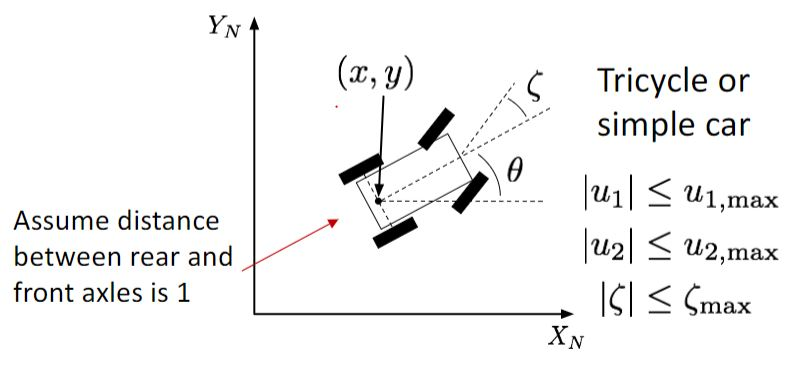
\includegraphics[width=0.4\textwidth]{tricycle}
\caption{Tricycle Model}
\end{figure}

The kinematic model of tricycle robots is as follows:

\[ \begin{pmatrix}
\dot{x} \\ \dot{y} \\ \dot{\theta} \\ \dot{\xi}
\end{pmatrix} =
\begin{pmatrix} \cos \xi \cos \theta \\ \cos \xi \sin \theta \\ \sin \xi \\ 0 \end{pmatrix} u_1 + \begin{pmatrix} 0 \\ 0 \\ 0 \\ 1 \end{pmatrix} u_2
\]

\textbf{Warning:} A kinematic state space model should only be interpreted as a subsystem of a more general dynamical model of the robot.

You control the robot by controlling actual forces and torques, not linear and angular speeds. Usually we assume that there is a black box that converts desired angular and linear velocities to actual torques on each wheel. Alternatively, we could reason directly with the dynamical model, but we won't do this until later in the class.

\subsection*{Simplified car models}

Assuming we do not care about the direction of the front wheels, we can set $v = u_1 \cos \xi$, and $w = u_1 \sin \xi$, and plug these two equalities into our kinematic model of the tricycle model, yielding:

\begin{center}
$
\begin{pmatrix}
\dot{x} \\ \dot{y} \\ \dot{\theta} \\ \dot{\xi}
\end{pmatrix} =
\begin{pmatrix} \cos \xi \cos \theta \\ \cos \xi \sin \theta \\ \sin \xi \\ 0 \end{pmatrix} u_1 + \begin{pmatrix} 0 \\ 0 \\ 0 \\ 1 \end{pmatrix} u_2
$ $\Rightarrow$ $
\begin{pmatrix}
\dot{x} \\ \dot{y} \\ \dot{\theta}
\end{pmatrix} =
\begin{pmatrix} \cos \theta \\ \sin \theta \\ 0 \end{pmatrix} v + \begin{pmatrix} 0 \\ 0 \\ 1 \end{pmatrix} w
$
\end{center}

As it can clearly be seen, this assumption has reduced our simple car-like system to the equivalent kinematic representation of the unicycle model. Of note, however, is that while the kinematic model reduces to become indiscriminate of the unicycle model, there is a coupling of the constraints that changes the behavior of the vehicle.

Below are a few examples of how the relationship of $v$ and $w$ relate to $u_{1,max}$ \cite{jp}:
\\\\
$
|v| \leq u_{1,max}\;\textup{cos}(\zeta_{max}),\;|w|\leq |v|\;\textup{tan}(\zeta_{max}) \rightarrow \textup{Car-like robot}
$

$
|v|= u_{1,max}\;\textup{cos}(\zeta_{max}),\;|w|\leq |v|\;\textup{tan}(\zeta_{max}) \rightarrow \textup{Reeds \& Shepp's car}
$

$
v= u_{1,max}\;\textup{cos}(\zeta_{max}),\;|w|\leq |v|\;\textup{tan}(\zeta_{max}) \rightarrow \textup{Dubin's car}
$

\section*{Further Readings and Additional Resources}

\begin{itemize}
   \item  Additional information on holonomic vs. nonholonomic constraints
   \begin{itemize}
     \item  \url{https://alliance.seas.upenn.edu/~meam535/cgi-bin/pmwiki/uploads/Main/Constraints10.pdf}
     \item \url{http://www.cs.cmu.edu/afs/cs/academic/class/16741-s07/www/lectures/lecture5.pdf}
   \end{itemize}
   \item PowerPoint slides on dynamics, wheels, and constraints
   \begin{itemize}
     \item  \url{http://www.csc.kth.se/utbildning/kth/kurser/DD2426/robot-h08/mtrl/Kinematics2x2.pdf}
   \end{itemize}
   \item Rotation Matrices Review
   \begin{itemize}
       \item \url{http://mathworld.wolfram.com/RotationMatrix.html}
   \end{itemize}
 \end{itemize}


\begin{thebibliography}{9}

\bibitem{ssvo}
B. Siciliano, L. Sciavicco, L. Villani, G. Oriolo.\textit{ Robotics: Modelling, Planning, and Control.} \\Springer, 2008 (chapter 11).

\bibitem{sns}
R. Siegwart, I. R. Nourbakhsh, D. Scaramuzza. \textit{Introduction to Autonomous Mobile Robots.} MIT Press, 2nd Edition, 2011.

\bibitem{jp}
J.-P. Laumond. \textit{Robot Motion Planning and Control.} 1998 \\texttt{https://homepages.laas.fr/jpl/promotion/chap1.pdf}

\bibitem{swed}
L. Lin, H. Shih. \textit{Modeling and Adaptive Control of an Omni-Mecanum-Wheeled Robot.} \\Intelligent Control and Automation, 4, 166-179. doi: 10.4236/ica.2013.42021.

\end{thebibliography}

\subsubsection*{Contributors}
Winter 2019: S. Bernardon, T. DeWeese,  A. Jagesten, P. Pipatpinyopong, G. Spellman, J. Malmstrom, M. Ricks, and V. Zhang
\\
Winter 2018: S. Spears, C. Covert, A. Hosler, Z. Chase, and H.M. Ewald

\end{document}
